\documentclass[twocolumn,11pt]{article}
\setlength{\textheight}{9truein}
\setlength{\topmargin}{-0.9truein}
\setlength{\parindent}{0pt}
\setlength{\parskip}{10pt}
\setlength{\columnsep}{.4in}

\usepackage{amsmath,amsfonts,amssymb,amsthm,bm,caption,calc,ifthen,graphicx,url,hyperref}

\begin{document}
\pagestyle{plain}
\onecolumn
PHYS689 
\newline Homework 5
\newline Will Wainwright
\newline Repository: \href{https://github.com/wjwainwright/PHYS689}{https://github.com/wjwainwright/PHYS689}

\section*{Discussion}
The procedure that I used involved generating data with a source function, applying noise to that data, and then using the normal method to fit the data. To generate the data, I used a generic polynomial function that can take any number of coefficients. For the most simple case, I used a linear model with $a_1=5$ and $a_0=7$. I generated random, Gaussian noise with a mean of zero and a standard deviation of one. I added this noise to the signal and then calculated the signal to noise ratio at the last point. With the target SNR being 3, I then scaled the noise so that the new SNR at the last point was 3, and added it to the signal. I used the same process to generate the data set for the second part of the homework, using a different function.

With the data set made and noise added, I first tested the fit using scipy's curve fit method. I then wrote my own normal method function which takes arrays of x values and the ``measured'' signal with noise at those points. The function also takes a list of uncertainties for the points, which in my case I took to be uniform. From my understanding of the normal method, I then had to generate the design matrix whose elements were essentially the terms of the equation I was trying to fit but without coefficients. While I could have generated a simple linear design matrix, I choose to adopt the extra challenge of making it work for a variable number of polynomial terms. While I have not attached any plots of the higher order terms being fit, I tested up to a 4th degree polynomial and got pretty good results from the fit. Once the design matrix is constructed, I just perform a few matrix operations as shown in lecture, and then return the fit parameters and variance matrix. The diagonal elements of the variance matrix are the individual variances of the fit parameters. Comparing the fit from my normal method to that of scipy, both fits return the same fit parameters, but my normal method reports a much lower error, which has me skeptical. I think I may have populated the noise matrix incorrectly, but I'm not sure how else I would do it.

\begin{figure}[!h]
	\centering
	\noindent
	\makebox[\textwidth]{
      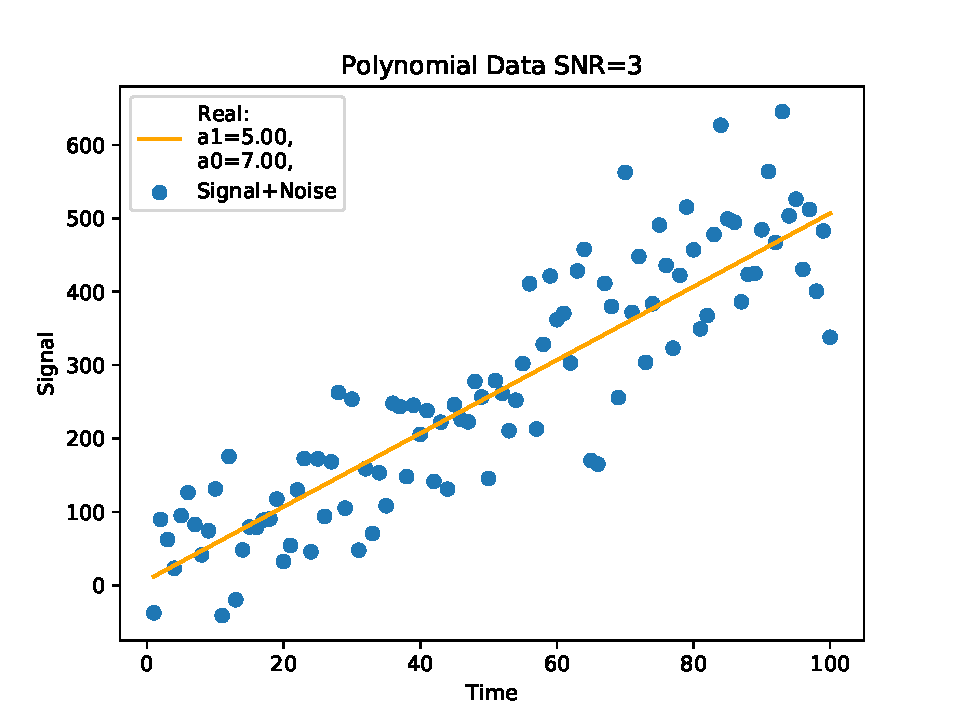
\includegraphics[width=5in]{polynomial.pdf}}
      \caption{Polynomial, in this case linear with $a_1=5$ and $a_0=7$.}
\end{figure}

\begin{figure}[!h]
	\centering
	\noindent
	\makebox[\textwidth]{
      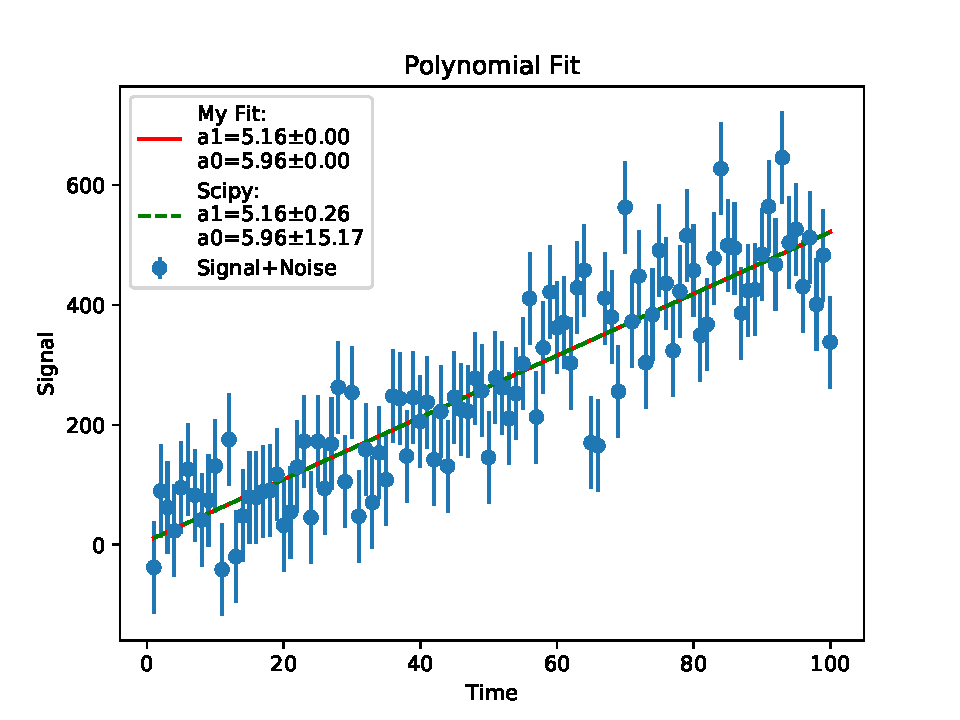
\includegraphics[width=5in]{polynomialFit.pdf}}
      \caption{Polynomial fit comparing the normal method to scipy.}
\end{figure}

For part two, in the case of a nonlinear function, I first experimented with exponential functions. I wanted to do something of the form of $a_ie^{x^i}$, but eventually I was restricted because the values were quickly overflowing. I ultimately settled on a function of the form $y=a_2x^2+a_1x+a_0+a_{-1}x^{-1}+a_{-2}x^{-2}$, with a variable number of terms being accepted, similar to my regular polynomial case. Creating the design matrix was the hardest part about using this function, as I had to map from a loop through the matrix to a loop from $-n$ to $n$. I also made some fancy strings for displaying the values as plot labels. One thing I noticed through both parts is that the spread on the data points, and therefore the goodness of fit, is highly dependent on whether the last data point is generated with a high or low random noise. Because the signal to noise is fixed by the last point, the scaling applied the the noise array as a whole depends on this dice roll.

\begin{figure}[!h]
	\centering
	\noindent
	\makebox[\textwidth]{
      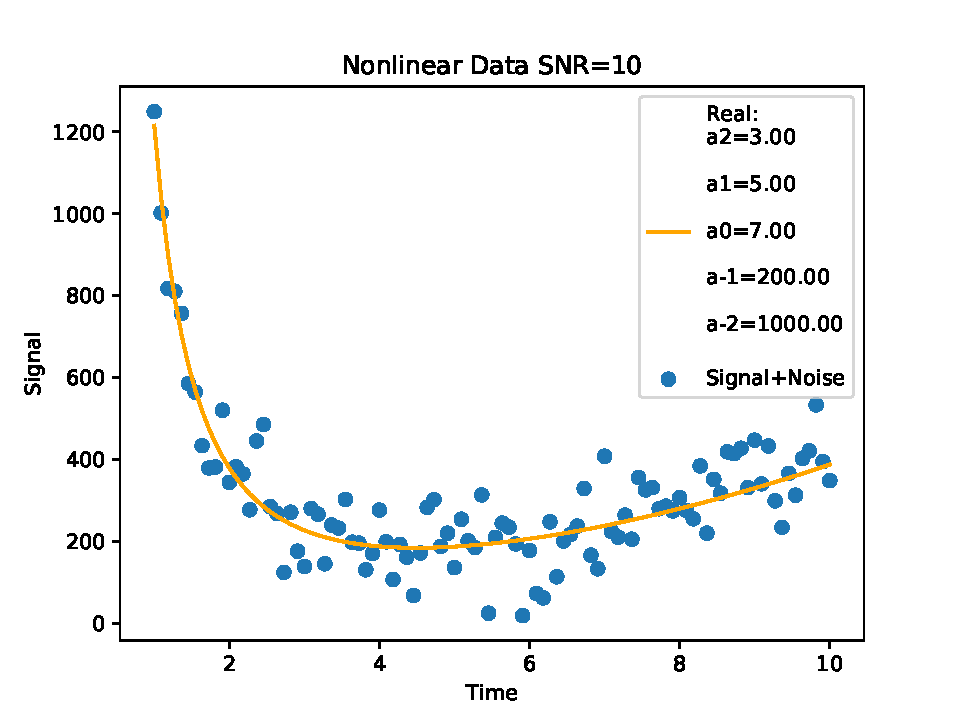
\includegraphics[width=5in]{nonlinear.pdf}}
      \caption{Nonlinear method following $y=a_2x^2+a_1x+a_0+a_{-1}x^{-1}+a_{-2}x^{-2}$.}
\end{figure}

\begin{figure}[!h]
	\centering
	\noindent
	\makebox[\textwidth]{
      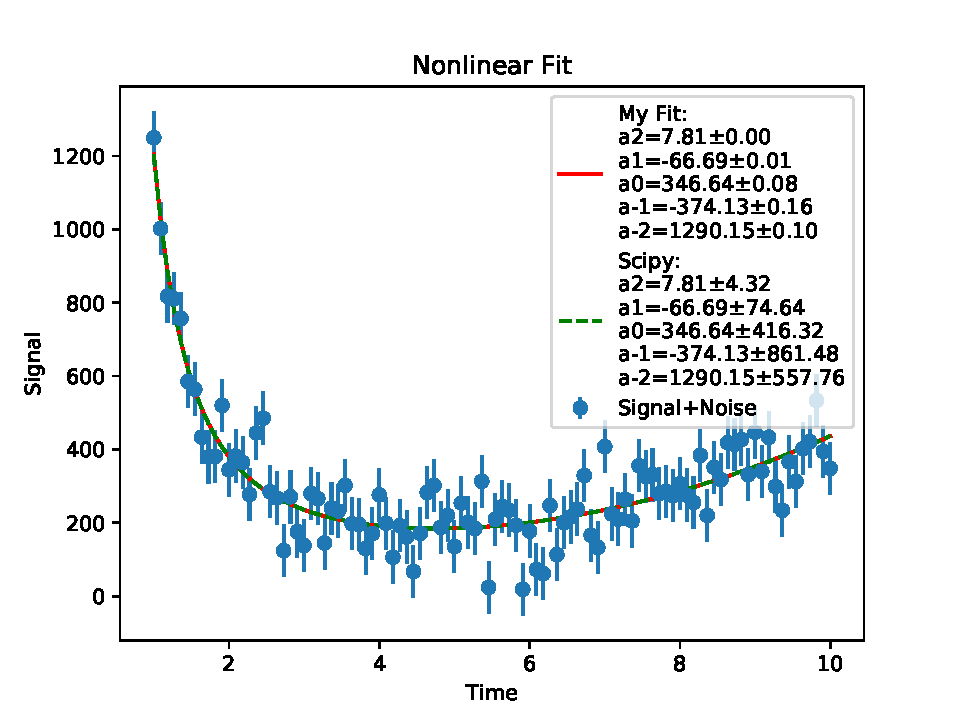
\includegraphics[width=5in]{nonlinearFit.pdf}}
      \caption{Nonlinear fit comparing the normal method to scipy.}
\end{figure}


Altogether, I had a lot of fun with this assignment, and learned some new things along the way, both about functions and fitting as well as about python. One thing I was unfortunately not able to accomplish was finding the probability to exceed for the given fits. I was able to calculate the $\chi^2$ values for the fits, but none of the packages I could find would take a pre-calculated $\chi^2$ and return a p-value. That being said, I'm still pleased with what I accomplished and impressed with how effective a few matrix operations are at fitting a data set. The hardest part seems to be effectively constructing the design matrix.

\end{document}